\RequirePackage{plautopatch}
\documentclass[upLaTeX,a4paper]{jsarticle}
\usepackage{listings,jlisting,amsmath,otf,here,empheq}
\usepackage[dvipdfmx,dvips]{graphicx}

\lstset{
breaklines = true,
numbers = left,
frame = tbrl,
tabsize = 4,
captionpos = t
}

\title{流体の数値計算プログラムの作成 修正レポート}
\author{B4 津田修一朗}
\date{2021/6/15}

\begin{document}
\maketitle

具体的な手法については前回、前々回のレポートで述べたため、このレポートでは前回レポートからの修正点を中心に議論する。

\section{数値計算の手順,手法}
\subsection{流れ関数と渦度を求めるプログラムの実装}
流れ関数-渦度法により,cavity内の流れを解いた.
差分方程式の実装に誤りが合ったため修正した。

また、これまでは流れ関数$\varPsi$渦度$\omega$の収束条件を,すべての格子点において
\begin{equation}
  |\varPsi^n_{i,j}-\varPsi^{n-1}_{i,j}| < 0.0001  かつ  |\omega^n_{i,j}-\omega^{n-1}_{i,j}| < 0.0001
\end{equation}
が成り立つとしていたが,
\begin{equation}
  |\varPsi^n_{i,j}-\varPsi^{n-1}_{i,j}| < 0.00001  かつ  |\omega^n_{i,j}-\omega^{n-1}_{i,j}| < 0.00001
\end{equation}
に変更した。
これにより、流線図においてcavity底面付近の逆流渦が大きくなったことが確認されたため,前回までの収束条件では十分に収束できていなかったと考えられる.

しかし、収束条件を厳しくした結果,格子点$151 × 151$に設定した時にはプログラムを実行してから30分程度経過しても収束条件を満たさなかった。
そのため,今回は(i)レイノルズ数$Re = 50$, 格子点$51\times 51$, (ii)レイノルズ数$Re = 200$, 格子点$101\times 101$
でシミュレーションを行った.

\subsection{速度ベクトル図の描画}
速度ベクトルは, x = 0, 0.02, . . . 0.98, 1, y = 0, 0.02, . . . 0.98, 1 上の格子点のものを描画した.
また,cavity底面付近の逆流渦の挙動を確認する為に、各格子点における速度ベクトルをその大きさで割り,
流れの方向が分かりやすくなるようにした図を追加した.

\subsection{等圧線図の描画}
前回までは圧力のポアソン方程式を用いた差分方程式により圧力場を求めていたが,確からしい結果が得られなかったため,\cite{2}で紹介された方法を用いた.
無次元化された定常流のNavier-Stokes方程式は,

\begin{equation}
  \begin{split}
    u\frac{\partial u}{\partial x} + v\frac{\partial u}{\partial y} & = - \frac{\partial p}{\partial x} + \frac{1}{Re}\left( \frac{\partial^2 u}{\partial x^2} + \frac{\partial^2 u}{\partial y^2} \right) \\
    u\frac{\partial v}{\partial x} + v\frac{\partial v}{\partial y} & = - \frac{\partial p}{\partial y} + \frac{1}{Re}\left( \frac{\partial^2 v}{\partial x^2} + \frac{\partial^2 v}{\partial y^2} \right) \\
  \end{split}
\end{equation}
であり,これを変形し,
\begin{equation}
  \begin{split}
    \frac{\partial p}{\partial x} & = \frac{1}{Re}\left( \frac{\partial^2 u}{\partial x^2} + \frac{\partial^2 u}{\partial y^2} \right) - u\frac{\partial u}{\partial x} - v\frac{\partial u}{\partial y}\\
    \frac{\partial p}{\partial y} & = \frac{1}{Re}\left( \frac{\partial^2 v}{\partial x^2} + \frac{\partial^2 v}{\partial y^2} \right) - u\frac{\partial v}{\partial x} - v\frac{\partial v}{\partial y}\\
  \end{split}
\end{equation}

差分方程式は
\begin{equation}
  \begin{split}
    p_{i,j} = & p_{i-1,j} + \frac{1}{Re} \left( \frac{u_{i+1, j} + u_{i,j+1} + u_{i-1, j} + u_{i,j-1} - 4u_{i,j}}{h} \right) \\
     & - u_{i,j} \frac{u_{i+1,j}-u_{i-1}}{2} - v_{i,j}\frac{u_{i,j+1}-u_{i,j-1}}{2}
  \end{split}
\end{equation}
\begin{equation}
  \begin{split}
  p_{i,j} = & p_{i,j-1} + \frac{1}{Re} \left( \frac{v_{i+1, j} + v_{i,j+1} + v_{i-1, j} + v_{i,j-1} - 4v_{i,j}}{h} \right) \\
  & - u_{i,j} \frac{u_{i+1,j}-u_{i-1}}{2} - v_{i,j}\frac{u_{i,j+1}-u_{i,j-1}}{2}
  \end{split}
\end{equation}
とし,点(0,0)のにおける圧力$p=0$とした.
境界条件は
\begin{empheq}{alignat=2}
  \frac{\partial p}{\partial x} = 0 \quad (x=0, 1) \\
  \frac{\partial p}{\partial x} = 0 \quad (y=0,1)
\end{empheq}
であり,点(h,0),(0,h),(h,h)における圧力も$p=0$とおける.
計算手順は
\begin{enumerate}
  \item $x=h$上の圧力を式()により求める
  \item 1.で求めた圧力値を起点として、式()より壁面以外の残りの点の圧力を求める
  \item 境界条件により,壁面上の圧力値を求める
\end{enumerate}
とした.


\section{数値計算の結果}
\subsection{速度ベクトル図}
図1,2,3に今回得られた速度ベクトル図を示す.これらの図より,$(0,1),(1,1)$間を結ぶ線分に相当する移動壁面付近で比較的速い流れが生じ,cavity内に1つの渦ができていることが確認できる.
また,レイノルズ数$Re$が大きくなるにつれて、渦の中心が点(1, 1)に近づくことが確認できる.
さらに,レイノルズ数$Re=500$のときには$y=0$付近で流体の速さがおおよそ0であることがわかった.
\begin{figure}[H]
  \centering
  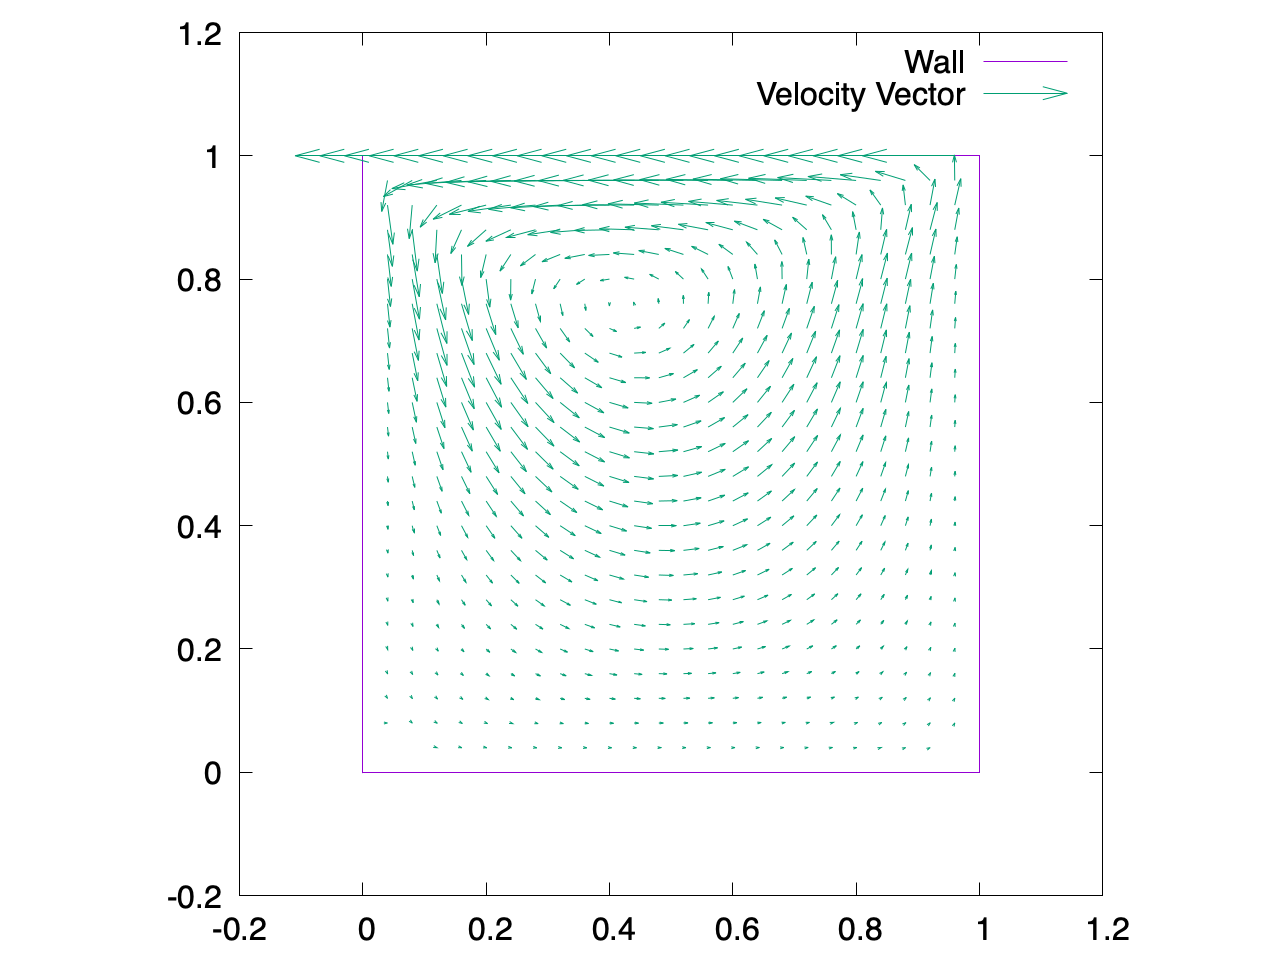
\includegraphics[height=9.5cm]{outputs/img/velocity_vector_re50.png}
  \caption{速度ベクトル図(i)}
  \label{fig:velocity_vector_re50}
\end{figure}
\begin{figure}[H]
  \centering
  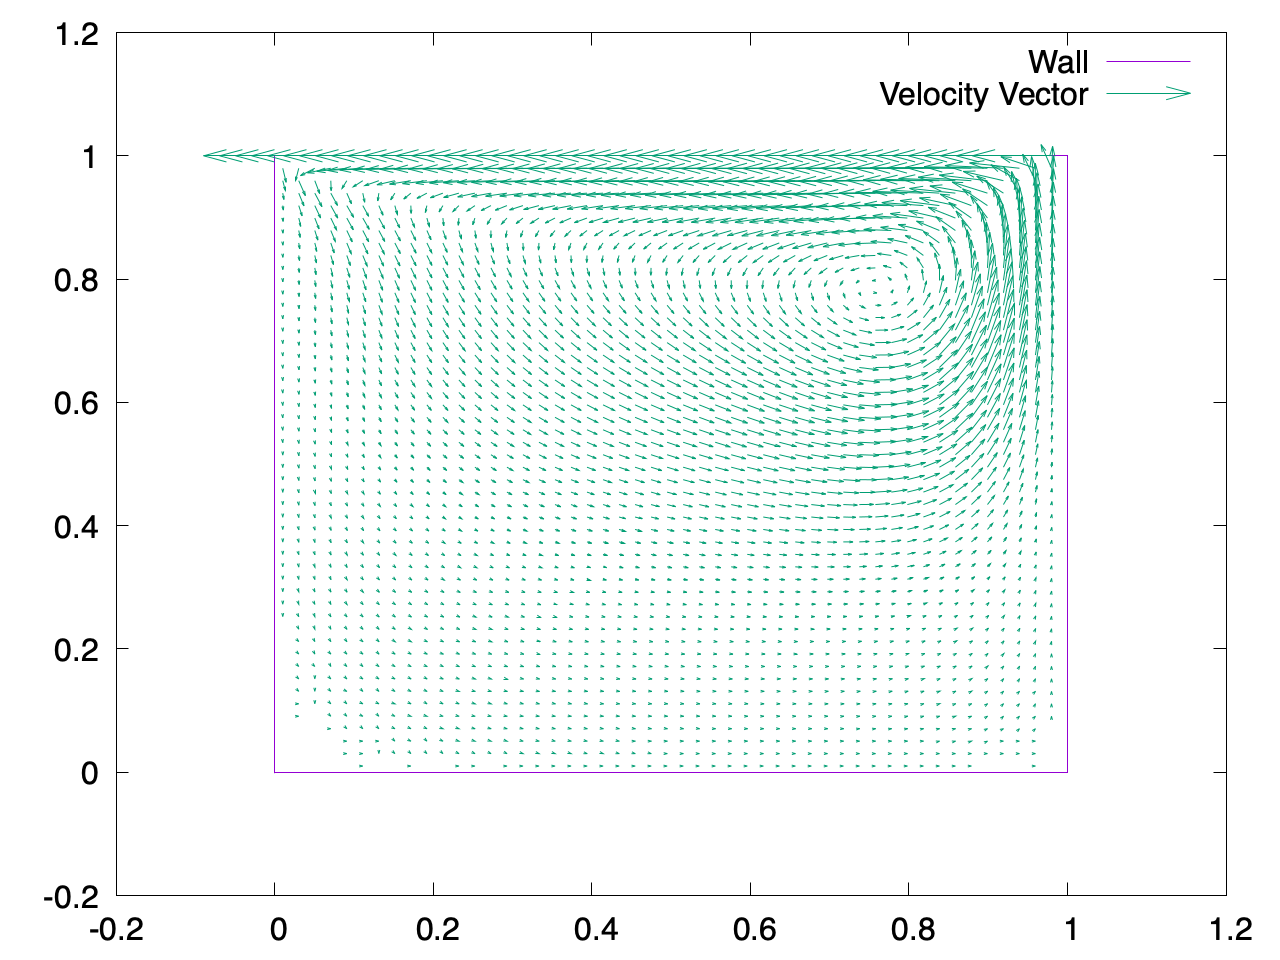
\includegraphics[height=9.5cm]{outputs/img/velocity_vector_re200.png}
  \caption{速度ベクトル図(ii)}
  \label{fig:velocity_vector_re200}
\end{figure}


\subsection{流線図}

図4,5,6に今回得られた流線図を示す.
中間報告においては, gnuplotの格子状データを生成するdgrid3d機能を用いていたため,比較的離れた格子点の情報が入ってしまっていた.
しかし,その後データを格納しているcsvファイルの形式を修正し,dgrid3dを使わず,数値解析によって得られた値をそのまま格子状データとして描画する方法を用いたので,最近接点のみの情報で表現できた.

\begin{figure}[H]
  \centering
  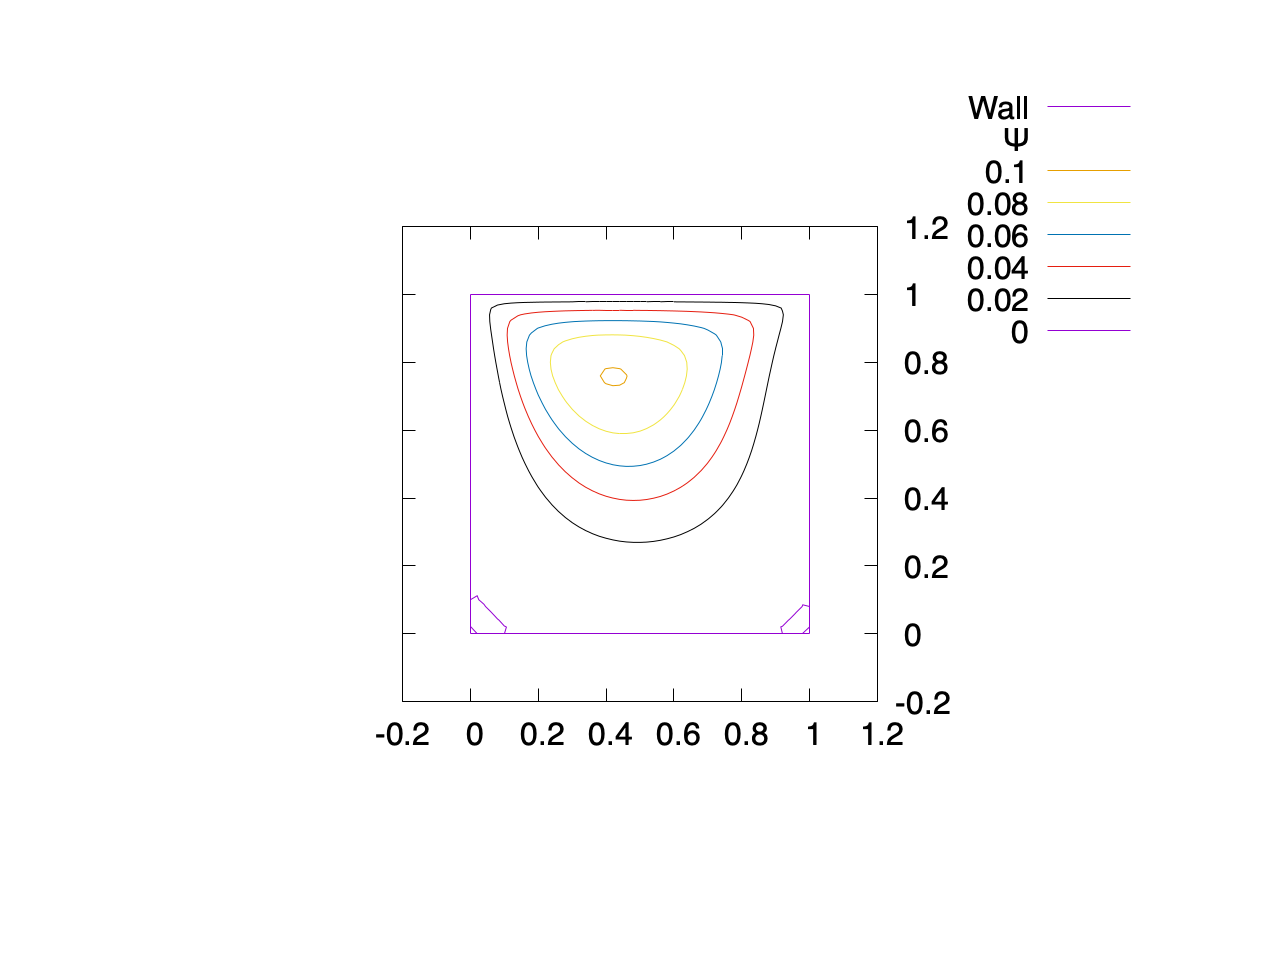
\includegraphics[height=9.5cm]{outputs/img/stream_line_re50.png}
  \caption{流線図(i)}
  \label{fig:velocity_vector_re50}
\end{figure}
\begin{figure}[H]
  \centering
  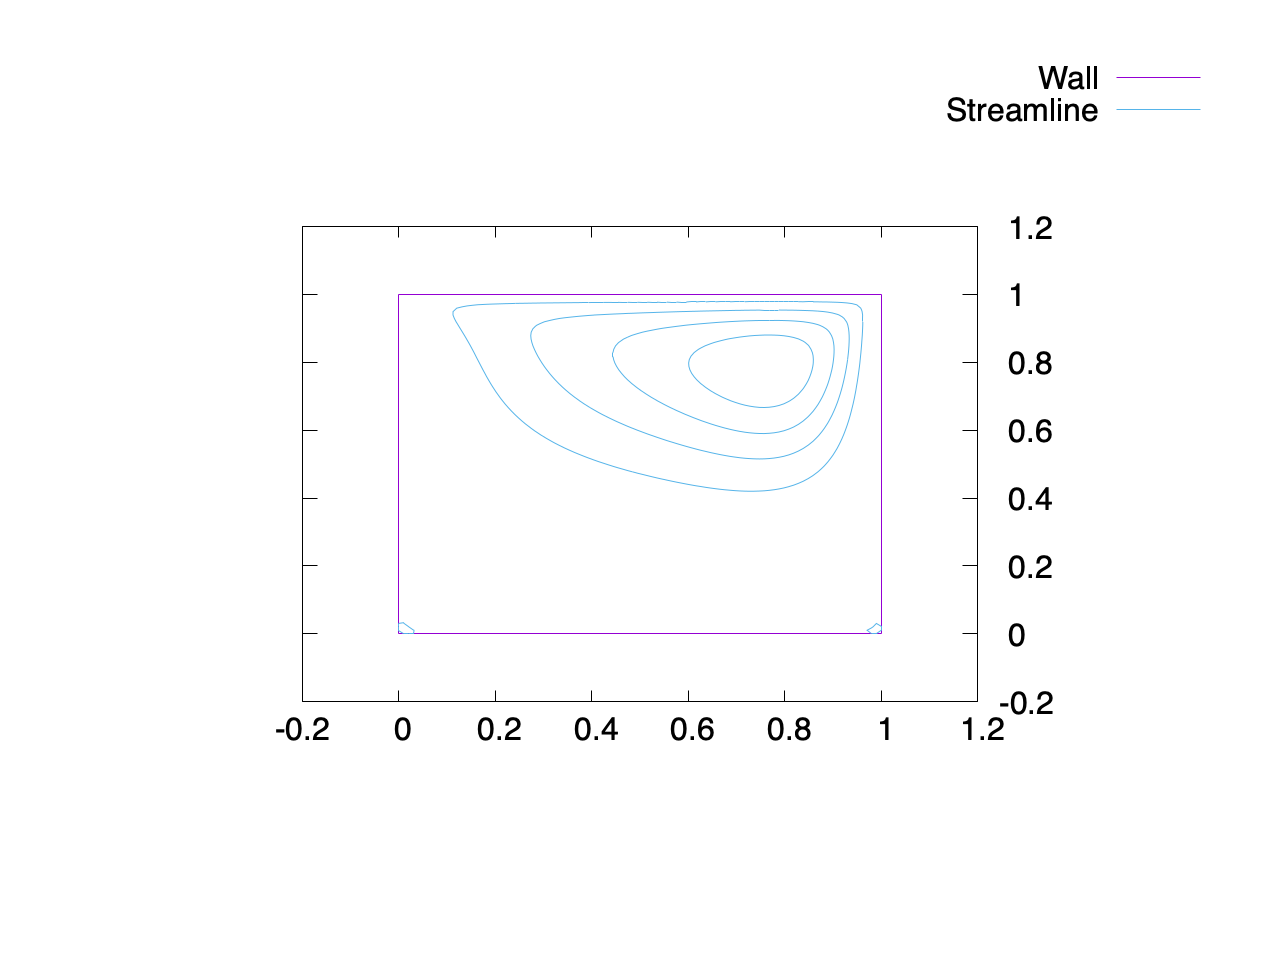
\includegraphics[height=9.5cm]{outputs/img/stream_line_re200.png}
  \caption{流線図(ii)}
  \label{fig:velocity_vector_re200}
\end{figure}


\subsection{等圧線図}
図7,8,9に今回得られた等圧線図を示す.
$(0,0),(1,0)$を結ぶ線分付近で圧力が高く,点(0,1),(1,1)付近で圧力が低い結果となった.
\begin{figure}[H]
  \centering
  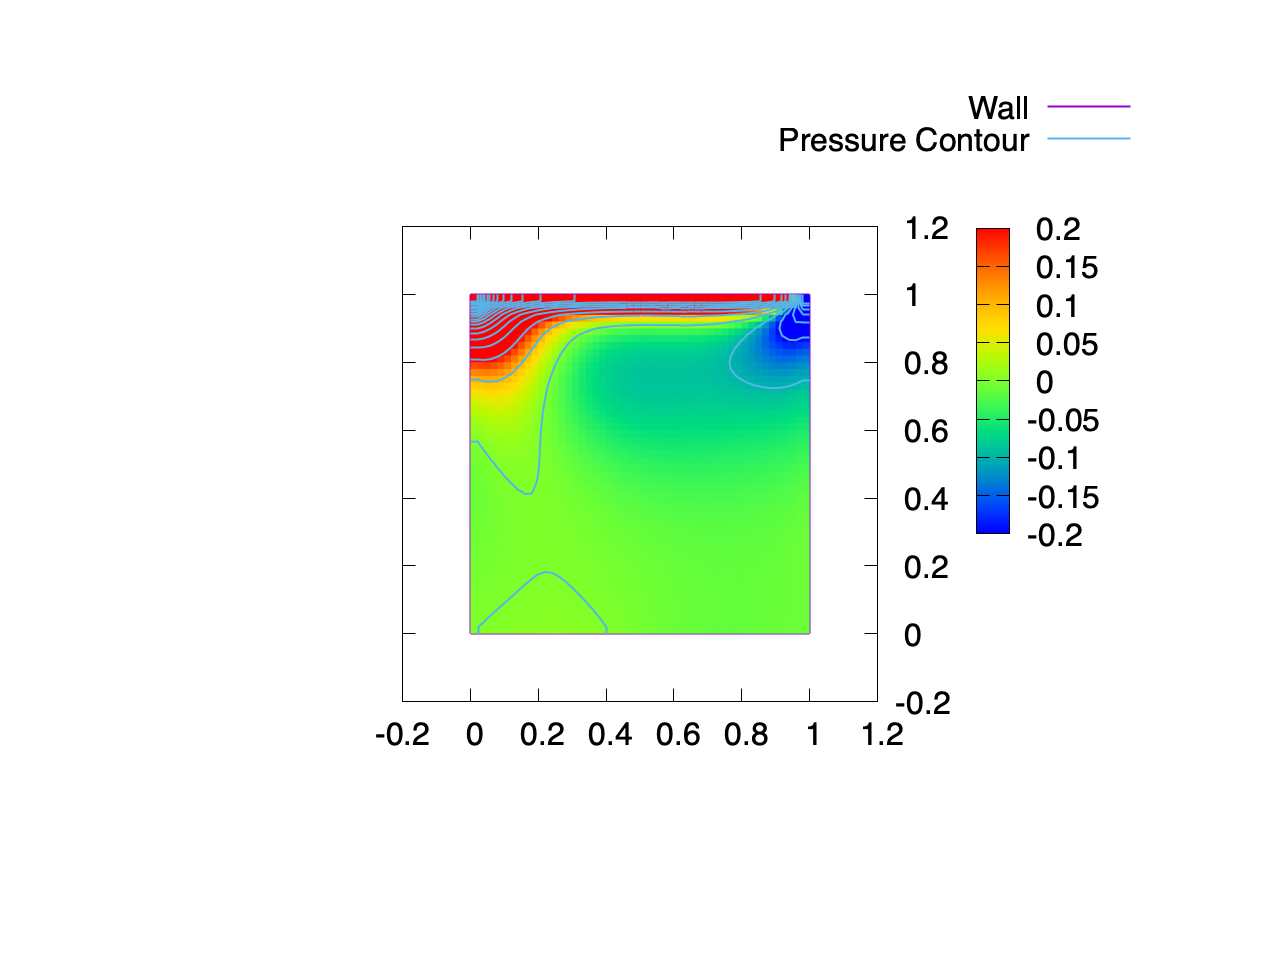
\includegraphics[height=9.5cm, clip,trim=0 200 0 0]{outputs/img/p_re50.png}
  \caption{等圧線図(i)}
  \label{fig:p_re50}
\end{figure}
\begin{figure}[H]
  \centering
  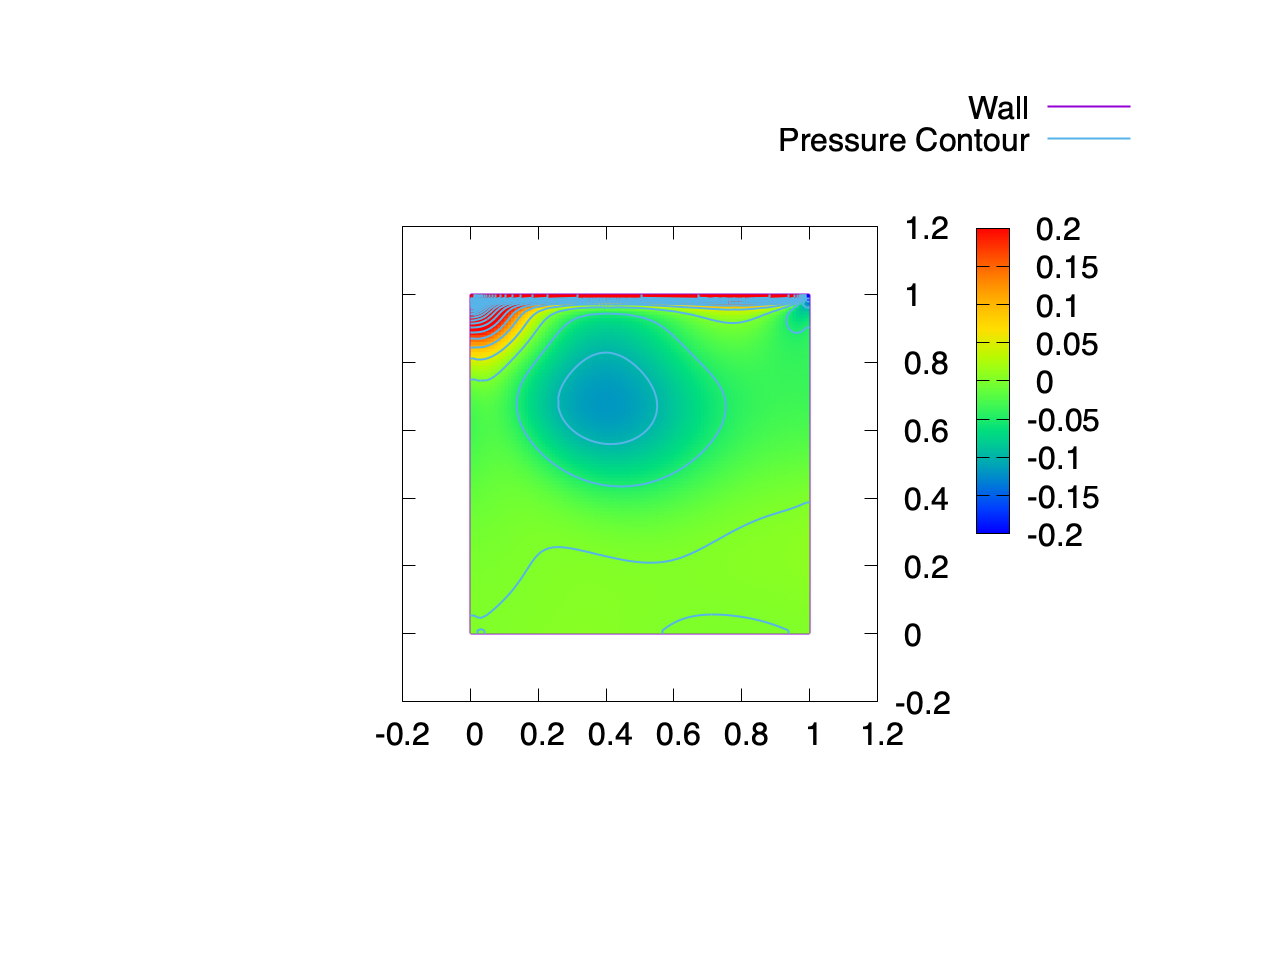
\includegraphics[height=9.5cm, clip,trim=0 200 0 0]{outputs/img/p_re200.png}
  \caption{等圧線図(ii)}
  \label{fig:p_re200}
\end{figure}

\begin{thebibliography}{9}
  %	\bibitem{1} \url{http://www.hal.t.u-tokyo.ac.jp/lab/ja/index_1.xhtml}
  %    \bibitem{2}Olga Russakovsky*, Jia Deng*, Hao Su, Jonathan Krause, Sanjeev Satheesh, Sean Ma, Zhiheng Huang, Andrej Karpathy, Aditya Khosla, Michael Bernstein, Alexander C. Berg and Li Fei-Fei. (* = equal contribution) ImageNet Large Scale Visual Recognition Challenge. IJCV, 2015.
  \bibitem{1} 研究室資料.流体の数値計算(川口光年先生1976年頃).pdf
  \bibitem{2} 越馬 遼 研究レポート (2021/6/17に提出されたもの)
\end{thebibliography}
\end{document}